% =====================================================================
% sections/algo_compare.tex — §5.9 算法比较（rev.1，2026-07-07 轻流程起草落地）
% 依据：spec §2 §5.9 块（两层结论顺序 + 口径红线）+ §0.4 红线 5 + §0.5.9/§0.5.10
%   + §5 图表清单 (5.9) 行 + next_session_prompt.md（轻流程：论点骨架直落）。
% 数字 ground truth（唯一权威，全部实时回查）：
%   docs/fql_succession_p2_results.md
%     §2（2×2 矩阵：E-uni R 0.885 / F 0.858(n=4) δ−0.027；M-uni-noise R 0.705 /
%         F 0.910 δ+0.205；E-multi R 0.810 / F 0.790 δ−0.020；M-multi-mix
%         R 0.990 / F 0.955 δ−0.035；门槛 |δ|≤0.03 / ≥0.05）
%     §3（Q1 0.705→0.715、Q 目标 −150→−123；Q1b 0.705→0.940 +23.5pp；
%         Q1c 0.885→0.910 +2.5pp；噪声轴网格 worst 0.705/0.910/0.858）
%     §4（C-1：0.3→0.740 / 1.0→0.858(n=4) / 3.0→0.790 / 10.0→0.855；
%         对照 0.910；−5.2pp）
%     §5（σ_train≈3.8pp、11 单元均距 4.3pp；t：+0.235→4.98、+0.205→8.20、
%         +0.055→0.88、+0.030→0.75、+0.025→0.82、n=4 复核 −0.052 t≈1.2；
%         df=2 临界 4.30）
%     §6（机制归因）§6.5（u15_cross FLOOR：0.985→0.719 / 0.632→0.098 /
%         offline 0.14、OOB 78/100、in-training ~0.09）§7（claim 边界）
%     §8.1（β1=4.0 主线口径四轴差异——本节只作线别限定，不 reconcile）
%   docs/arrival_v2_sac_collector_design.md §4.0.10（36-cell joint：
%     0.002/0.515/0.751/0.899 档；R1 0.656±0.069 / 0.800±0.033 / 0.889±0.019；
%     R4 0.633±0.067 / 0.711±0.038 / 0.889±0.019；FQL 0.733±0.100 /
%     0.922±0.038 / 0.911±0.019；CI：mexp FQL−R1 +0.123[+0.022,+0.233]、
%     medium +0.077[−0.056,+0.233]、aggregate +0.074[+0.015,+0.137]、
%     FQL−R4 mexp +0.212[+0.122,+0.311]、R1−R4 mexp +0.089[+0.011,+0.178]；
%     m_multi_mix 补充 0.987±0.006、R1−FQL +0.035[+0.010,+0.065]、
%     R1−R4 −0.000[−0.020,+0.025]）+ §4.0.1/§4.0.3/§4.0.7（四档检查点
%     2.5万/42.5万/57.5万/60万步、1M 总预算、随机策略采样、转移
%     180067/250544/171394/114832、回合均长 180/251/171/115）
%   docs/fql_succession_p2_collection_log.md（四单元构造与 1000 回合规模）
% 红线（spec §2 §5.9 + §0.4 红线 5 + prompt）：两层结论顺序不可倒；第一层
%   「ReBRAC-Q 占优」不作章级主结论；mexp 反超=同源可报效应量、翻转另一侧
%   （m_multi_mix）异源仅方向、不 claim 幅度比；u15_cross FLOOR 作 scope
%   caveat 不弱化主工况；FQL n=2 带 caveat 引用级、统计强度同台；β1=1.0 vs
%   4.0 不在本节 reconcile（就近线别限定一句，统一留 §5.10）；特权 critic
%   四态收束留 §5.10；禁 teacher 作概念主语（「流匹配模型积分去噪的参照动作/
%   蒸馏所得部署策略」）；数据 regime→数据条件/质量区间；报告体 marker 零出现。
% 本轮裁决（轻流程）：图 2 张新作（fig_ch5_fql_noise_axis 重绘噪声轴网格、
%   fig_ch5_algo_interaction 章级 headline interaction 图）+ 表 3 张（2×2 矩阵 /
%   C-1 扫描 / SAC 四档联合矩阵）；verdict matrix / c1-rescue 两图以表呈现。
%
% rev.2（2026-07-07）：独立对抗复审落地（findings 存档
%   section_5_9_review_findings.md；ground truth 全量回查含 p2_main_spec §5.5
%   预登记原文与 xbench spec，未采信任何成稿自述）。三表两图数字零漂移、红线
%   子集零踩线；修订实质项（0 CRIT / 4 HIGH / 8 MED / LOW 顺手 3 条）：
%   [HIGH-归属] 预登记主要正例 = 小噪多模态单元（spec v1.3 §5.5 主判原文 +
%     diagnostic §2；results.md §2 括注"E-multi primary"系孤例，按 diagnostic
%     为准），非干净多模态；"命中三分之一"三单元记账撤除，改写为四项预测仅
%     干净单模态一项成立、唯一方向性差异出现在被预测为无差异的含噪单模态。
%   [HIGH-机制前提] 小噪多模态解释"观测区域彼此错开"与 diagnostic §5
%     "mostly-overlapping trajectories"相反（E-multi 审计 p_≥2=0.182 佐证）
%     → 改"大范围重叠、同一观测下显著分歧动作很少"。
%   [HIGH-跨节指认] FLOOR 段"在另一工况参数点的重现"错误——xbench 与 §5.8
%     N2' 同为临界 u15 横流工况，独立的是配置(β1=1.0)/示范数据(新采)/评估集
%     (ep100)；"单点传感充分性边界"对齐 §5.8 自身口径 → 改"同一临界工况下
%     刻画的单点观测策略侧上限相互印证，两处证据彼此独立却触及同一边界"。
%   [HIGH-综合句] §5.9.5"含噪或中等质量…FQL 更优"与本节自身消融矛盾（含噪
%     单元 β1=1.0 0.940 ≥ FQL 0.910）→ 按 §4.0.10 质量区间口径重写（非饱和
%     中段同源占优 / 饱和高位至少相当且沿噪声轴更稳）。
%   [MED×8] 头对头括注统一 ReBRAC-Q 减 FQL 方向（+0.030/+0.055/n=4 后 +0.052，
%     撤字面为假的"同号"）；"稳健性优选而非均值优选"→"非单点最高值优选"
%     （对齐 §5.7.5，筛查表中 4.0 均值亦最高）；"以随机策略采样"→"保留检查
%     点策略随机动作采样"；FLOOR 补含噪采集器亚临界基线 0.632；"跨源补充
%     采集"→"补充训练"+ 配对种子集(两族共同两种子)就地声明；"预筛冻结"降
%     为"对照前冻结"（FQL α=1.0 系默认值未扫描，正文/表注/§5.9.m 三处）；
%     正文「」→全章弯引号“ ”；"SAC 中段质量档显著更优"收窄为中等偏专家档。
%   [LOW 顺手] mexp 差值改报配对自助均值差 +0.123（消 12.2/12.3 复算陷阱）；
%     "平均自举目标"→"训练日志中价值估计的平均水平"（P2 mean_q 与 §5.7 惩罚
%     前读取口径不同名同）；"最优方向且与…"语序；"高噪单元"统一为含噪单模态
%     单元。余 LOW×2（σ=0.5 事后加噪歧义已由 §5.9.m 澄清、图(a)参考线标记
%     描述）记录留收尾统稿轮。轻流程门控：CRIT+HIGH=4，触发 ≥4 呈报条件，
%     判定与建议见 findings §6（交用户拍板 §5.10 流程）。
% 收尾统稿轮（2026-07-08）：LOW 残留×2 已清——§5.9.1 σ=0.5 句改"在采集时对
%   行为策略的动作注入"（对齐 §5.9.m）；交互图 (a) caption 补"及其三角标记"。
%   零数字/零论证改动。
% =====================================================================

\section{算法比较：策略先验表达力与模仿目标的质量适配}\label{sec:ch5_algo_compare}

\S\ref{subsec:ch5_rebrac_implications} 把一个问题留给了算法比较：离线主线以原始数据动作为模仿目标，在高质量确定性示范上工作良好，而当行为数据含噪、多模态或质量下降时，这一模仿目标是否仍然恰当。生成式策略研究对此有一个通行预期——对原始动作的逐点回归难以覆盖多模态或次优的行为分布，先以生成式模型刻画该分布、再以其样本引导策略，应当在此类数据上占优~\citep{park2025fql}。\S\ref{subsec:ch5_method_fql} 定义的 FQL 恰好把这一预期收拢到一个干净的接口上：它与 ReBRAC-Q 同属确定性策略分支、共用 Q 归一化的价值改进项，两方法的结构差异集中在模仿项所指向的参照目标——原始数据动作，或流匹配模型积分去噪得到的参照动作 $\mathbf{a}_{\mathrm{FM}}$。比较这两个方法，检验的因此不是两套互不相干的算法，而是模仿目标这一单一接口在不同数据条件下的表现。

考察在两族数据来源上递进展开。全场走廊参照采集器一族把数据条件组织成受控矩阵并辅以单变量消融，判别两方法差异的机制来源；SAC 检查点采集器一族再以质量分档的数据阶梯，检验由此得到的排序是否随数据源保持。前者给出机制，后者划定该机制下算法排序的适用条件；本节的章级结论落在后者。

\subsection{对照假设与数据条件矩阵}\label{subsec:ch5_algo_matrix}

上述预期可操作化为一个可判假设：FQL 优于 ReBRAC-Q，当且仅当行为数据同时次优且多模态。假设的两个条件对应两条独立的数据轴——模态（单一行为策略，或两种行为策略的混合）与噪声（动作级噪声的有无）——以表~\ref{tab:ch5_datasets} 中全场走廊参照的亚临界到达导向高质量集为基准衍生出四个单元：基准本身构成干净单模态单元；在采集时对行为策略的动作注入 $\sigma=0.5$ 的高斯噪声得到含噪单模态单元；与目标直指参照按一比一混合得到干净多模态单元；在该混合上注入 $\sigma=0.1$ 小噪声得到小噪多模态单元。每个单元上两方法以完全相同的数据、传感与训练预算训练（配置在全部对照前冻结，\S\ref{subsec:ch5_algo_impl}），在主工况固定评估集上终检评估，判读门槛在实验前指定。

\begin{table}[t]
\centering
\caption{模态 $\times$ 噪声数据条件矩阵上的算法对照（成功率为跨随机种子均值，每种子终检 $100$ 回合；每单元两随机种子，干净单模态单元的 FQL 侧含后补共四种子）。两列均为对照前冻结的配置：ReBRAC-Q 取 $(\beta_1,\beta_2)=(4.0,\,2.0)$，FQL 取 $\alpha_{\mathrm{FQL}}=1.0$（\S\ref{subsec:ch5_algo_impl}）。判读门槛实验前指定：$|\delta|\le 0.03$ 判无差异，$|\delta|\ge 0.05$ 且各种子方向一致判方向性差异，其余判灰区。}
\label{tab:ch5_fql_matrix}
\small
\setlength{\tabcolsep}{5pt}
\begin{tabular}{l l c c c l}
\toprule
\textbf{单元} & \textbf{构成} & \textbf{ReBRAC-Q} & \textbf{FQL} & \textbf{$\delta$（FQL$-$R）} & \textbf{判读} \\
\midrule
干净单模态 & 全场走廊参照原集 & $0.885$ & $0.858$ & $-0.027$ & 无差异 \\
含噪单模态 & 原集 $+\ \sigma{=}0.5$ 动作噪声 & $0.705$ & $0.910$ & $+0.205$ & FQL 方向性占优 \\
干净多模态 & 与目标直指参照 $1{:}1$ 混合 & $0.810$ & $0.790$ & $-0.020$ & 无差异 \\
小噪多模态 & 混合 $+\ \sigma{=}0.1$ 噪声 & $0.990$ & $0.955$ & $-0.035$ & 灰区 \\
\bottomrule
\end{tabular}
\end{table}

矩阵的判读结果否定了假设的模态一侧（表~\ref{tab:ch5_fql_matrix}）。按该假设，混入示范质量明显更低的目标直指参照使两个多模态单元同时次优且多模态、都应给出 FQL 的方向性优势——小噪多模态单元更是实验前指定的主要正例——而结构上单模态的两个单元应无差异；实测恰好相反：唯一的方向性差异出现在被预测为无差异的含噪单模态单元（$\delta=+0.205$），干净多模态单元恰为无差异（$\delta=-0.020$），四项预测仅干净单模态一项成立——干净的多模态本身没有给生成式先验带来任何可检出的好处。作为主要正例的小噪多模态单元亦落在灰区且方向偏负（$\delta=-0.035$）：混合的两种行为策略所访问的观测区域大范围重叠，在同一观测下给出显著分歧动作的情形很少，加之每分量噪声仅 $\sigma=0.1$，行为克隆项在同一观测条件下实际面对的条件动作方差 $\mathbb{E}_{\mathbf{o}}[\mathrm{Var}(\mathbf{a}\mid\mathbf{o})]$ 依然很低。判别变量由此收敛为动作噪声的幅度而非模态数，“当且仅当次优且多模态”的假设被证伪。

但证伪假设并没有解释掉含噪单模态单元上那 $20.5$ 个百分点——它看起来仍是生成式先验的一场真实胜利。这一优势究竟是 FQL 的结构性质，还是对照配置的产物，须由受控消融回答。

\subsection{机制判别：模仿目标的质量决定锚定强度的最优取值}\label{subsec:ch5_algo_anchor}

ReBRAC-Q 在含噪单模态单元上的落后可能来自其两个行为约束面中的任何一个，价值一侧先被排除。同一含噪数据上把价值侧系数 $\beta_2$ 由 $2.0$ 置零，成功率仅由 $0.705$ 移到 $0.715$，而训练日志中价值估计的平均水平由约 $-150$ 上移至 $-123$——系数确在生效，但价值侧支持惩罚不是约束策略质量的瓶颈。

瓶颈在策略一侧的锚定强度。同一含噪数据上把 $\beta_1$ 由 $4.0$ 降到 $1.0$（$\beta_2$ 保持 $2.0$），成功率由 $0.705$ 升至 $0.940$（$+23.5$ 个百分点），反超 FQL 的 $0.910$；把同一调整放回干净基准单元，成功率也由 $0.885$ 升到 $0.910$——$\beta_1=1.0$ 在两轴同时更好，干净与含噪之间不存在权衡。图~\ref{fig:ch5_fql_noise_axis} 把三个固定配置沿噪声轴并置：单一固定的 ReBRAC-Q（$\beta_1=1.0$）在干净轴与含噪轴分别高出 FQL $5.2$ 与 $3.0$ 个百分点，沿噪声轴的最坏成功率 $0.910$ 对 $0.858$。

\begin{figure}[t]
    \centering
    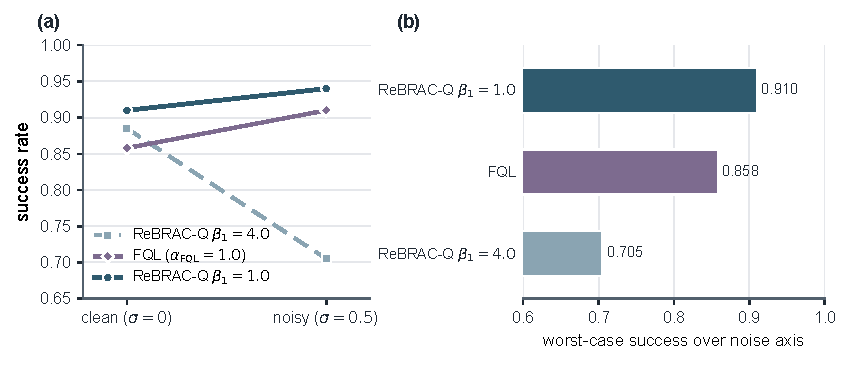
\includegraphics[width=138mm]{figures/fig_ch5_fql_noise_axis.pdf}
    \caption{锚定强度与模仿目标质量沿噪声轴的交互。(a) 三个固定配置在干净（$\sigma=0$）与含噪（$\sigma=0.5$）单模态单元上的终检成功率（每种子 $100$ 回合，跨种子均值）：ReBRAC-Q $\beta_1{=}4.0$ 在含噪数据上崩落（$0.885\to0.705$），$\beta_1{=}1.0$ 在两轴同时更好（$0.910/0.940$），FQL（蒸馏权重 $\alpha_{\mathrm{FQL}}{=}1.0$）居中且无需调整（$0.858/0.910$）。(b) 沿噪声轴的最坏成功率：$\beta_1{=}1.0$（$0.910$）$>$ FQL（$0.858$）$>$ $\beta_1{=}4.0$（$0.705$）。数字源自固定评估集终检，种子数见正文。}
    \label{fig:ch5_fql_noise_axis}
\end{figure}

这组消融把矩阵中唯一的正例溶解为一个可命名的机制。ReBRAC-Q 的模仿目标是原始数据动作：当数据动作携带不可约的注入噪声时，$\beta_1=4.0$ 的强锚定把确定性策略拖向噪声本身，削弱锚定即可恢复；FQL 的模仿目标是流匹配模型积分去噪后的参照动作，对称噪声下其条件均值即干净动作，故无需任何此类修正——而在干净数据上，这一去噪不再提供恰当加权的原始动作所没有的东西。同一族锚定系数、相反的最优方向，其取值由模仿目标是否含噪决定，与算法家族无关。

主线锁定的 $\beta_1=4.0$ 与此处的 $\beta_1=1.0$ 并不构成矛盾，但须作线别限定：两套协议在奖励设定、采集器、动作噪声与种子组四轴上均不同，且主线取值系跨种子稳健性优选而非单点最高值优选（\S\ref{subsec:ch5_rebrac_implications}）；两个最优取值在同一机制下的统一解释留待本章末节。

\subsection{对等调参复核与单一采集器族内的判定}\label{subsec:ch5_algo_rescue}

上一小节调整了 ReBRAC-Q 的锚定系数而 FQL 的蒸馏权重保持冻结，这一不对称在下判定前须先补平。复核在 FQL 的最坏轴——干净基准单元——上以对数间隔扫描其自身的锚定系数 $\alpha_{\mathrm{FQL}}$，并把冻结值单元补至四种子（表~\ref{tab:ch5_fql_c1}）。

\begin{table}[t]
\centering
\caption{FQL 蒸馏权重 $\alpha_{\mathrm{FQL}}$ 在干净基准单元上的对数间隔扫描（终检每种子 $100$ 回合），以同单元 ReBRAC-Q $\beta_1{=}1.0$ 为对照水平。}
\label{tab:ch5_fql_c1}
\small
\setlength{\tabcolsep}{6pt}
\begin{tabular}{l l c c}
\toprule
\textbf{配置} & \textbf{逐种子成功率} & \textbf{均值} & \textbf{种子数} \\
\midrule
$\alpha_{\mathrm{FQL}}=0.3$ & $0.75$、$0.73$ & $0.740$ & $2$ \\
$\alpha_{\mathrm{FQL}}=1.0$（冻结值） & $0.80$、$0.91$、$0.91$、$0.81$ & $0.858$ & $4$ \\
$\alpha_{\mathrm{FQL}}=3.0$ & $0.86$、$0.72$ & $0.790$ & $2$ \\
$\alpha_{\mathrm{FQL}}=10.0$ & $0.86$、$0.85$ & $0.855$ & $2$ \\
\midrule
ReBRAC-Q $\beta_1=1.0$（对照） & $0.88$、$0.94$ & $0.910$ & $2$ \\
\bottomrule
\end{tabular}
\end{table}

扫描没有找到能越过对照水平的取值。削弱锚定（$\alpha_{\mathrm{FQL}}=0.3$）使成功率大幅跌至 $0.740$，增强到 $10.0$ 也只回到 $0.855$ 的平台，最优仍在冻结值附近（四种子均值 $0.858$），距 ReBRAC-Q $\beta_1=1.0$ 的 $0.910$ 尚差 $5.2$ 个百分点。不仅水平不及，最优方向也与 ReBRAC-Q 相反——那一侧削弱锚定获益，这一侧削弱锚定受损——恰因 FQL 的参照动作本已干净，放松对它的对齐只是丢弃一个好目标。复核的失败因此不是机制的反例，而是它的再一次确认：锚定强度的最优点跟随模仿目标的质量，而非算法家族。

至此，全场走廊参照数据族内的判定完整：对等调参之下，单一固定的 ReBRAC-Q（$\beta_1=1.0$）在干净与含噪两轴都不低于 FQL，且沿噪声轴的最坏情形严格更稳。统计强度与证据规模同台交代：固定评估集使全部比较在相同任务实例上配对，种子间离散即纯训练种子方差（跨十一个单元的平均种子间距 $4.3$ 个百分点，折合 $\sigma\approx3.8$ 个百分点）；承载机制的两个大效应在每组两种子下即越过显著性门槛（$\beta_1$ 降档 $+0.235$，$t=4.98$；FQL 对 $\beta_1=4.0$ 为 $+0.205$，$t=8.20$；自由度 $2$ 的临界值 $4.30$），而 $\beta_1=1.0$ 与 FQL 之间的全部头对头差异均未过检出门槛、点估计一致偏向 ReBRAC-Q（以 ReBRAC-Q 减 FQL 计：含噪 $+0.030$，$t=0.75$；干净在两种子下 $+0.055$，$t=0.88$，FQL 侧补至四种子后为 $+0.052$，$t\approx1.2$，方向不变）。证伪一个优越性主张只需要“不赢”；追加种子会收紧这些无差异区间，而不会翻转其方向。

这一判定的效力边界同样清楚。它建立在单一采集器族之上——全场走廊参照及其受控变体——数据质量或处高位、或以人工注入的方式偏离；若算法排序真由模仿目标与数据质量的适配决定，换一族质量自然分档的数据源，排序就应当随之移动。这正是下一小节的检验，本节结论的真正落点在那里，而不在本小节的族内占优。

\subsection{跨数据源检验：算法排序随数据质量翻转}\label{subsec:ch5_algo_crosssource}

SAC 检查点采集器族（\S\ref{subsec:ch5_datasets}）提供了规则型采集器给不出的质量阶梯：沿一条在线 SAC 训练轨迹截取四个阶段的检查点作为行为策略，沿用离线强化学习基准按训练阶段分档构造数据的通行做法~\citep{fu2020d4rl}，四档采集器自身成功率从 $0.002$（随机档）经 $0.515$（中等档）、$0.751$（中等偏专家档）升到 $0.899$（专家档）。三个固定配置——ReBRAC-Q $\beta_1\in\{1.0,\,4.0\}$ 与 FQL——各以三随机种子在每档训练，连同小噪多模态单元的跨源补充共三十九个训练与评估运行（表~\ref{tab:ch5_algo_sac}；协议见 \S\ref{subsec:ch5_algo_impl}）。

\begin{table}[t]
\centering
\caption{SAC 检查点四档数据上的算法对照（成功率为三随机种子均值 $\pm$ 跨种子标准差，每种子终检 $30$ 回合；采集器成功率为各档一千回合采集时的实测值）。区间估计与关键对照的置信区间见正文。}
\label{tab:ch5_algo_sac}
\small
\setlength{\tabcolsep}{5pt}
\begin{tabular}{l c c c c}
\toprule
\textbf{档} & \textbf{采集器成功率} & \textbf{ReBRAC-Q $\beta_1{=}1.0$} & \textbf{ReBRAC-Q $\beta_1{=}4.0$} & \textbf{FQL} \\
\midrule
随机 & $0.002$ & $0.000 \pm 0.000$ & $0.000 \pm 0.000$ & $0.000 \pm 0.000$ \\
中等 & $0.515$ & $0.656 \pm 0.069$ & $0.633 \pm 0.067$ & $0.733 \pm 0.100$ \\
中等偏专家 & $0.751$ & $0.800 \pm 0.033$ & $0.711 \pm 0.038$ & $\mathbf{0.922 \pm 0.038}$ \\
专家 & $0.899$ & $0.889 \pm 0.019$ & $0.889 \pm 0.019$ & $0.911 \pm 0.019$ \\
\bottomrule
\end{tabular}
\end{table}

阶梯两端的信息量都有限：随机档三配置皆零，是质量阶梯的退化端点；专家档三配置全部收敛到采集器自身水平附近（$0.889$ 至 $0.911$），算法差异被数据上限吞没，属饱和区间。信息集中在中段——中等偏专家档上 FQL 达 $0.922\pm0.038$，对 ReBRAC-Q $\beta_1=1.0$ 的 $0.800\pm0.033$，分层配对自助的均值差 $+0.123$、$95\%$ 置信区间 $[+0.022,\,+0.233]$ 严格在零之上；中等档同方向（$+0.077$）但区间跨零，三个非退化档的聚合对照亦为 FQL 方向（$+0.074$，$[+0.015,\,+0.137]$）。在上一小节 ReBRAC-Q $\beta_1=1.0$ 双轴不低于 FQL 的地方，换成质量自然中等的数据源，同一对配置的排序发生了逆转。

在全场走廊参照一族、质量已然饱和的小噪多模态单元上，方向恰好相反：在该单元上补充训练的 ReBRAC-Q $\beta_1=1.0$（三随机种子）成功率 $0.987\pm0.006$，与同单元 FQL 在两族共同的两个随机种子上的逐回合配对差 $+0.035$、置信区间 $[+0.010,\,+0.065]$ 同样严格在零之上。两个方向相反的置信区间各自不含零——算法排序不是全局性质，而是随数据质量区间翻转（图~\ref{fig:ch5_algo_interaction}）。口径在此须精确：中等偏专家档的对照两侧同数据、同评估协议，效应量可直接报告；翻转的另一侧落在不同的数据集与评估协议上，跨数据源的比较只支撑方向读数，两侧幅度不可比。

\begin{figure}[t]
    \centering
    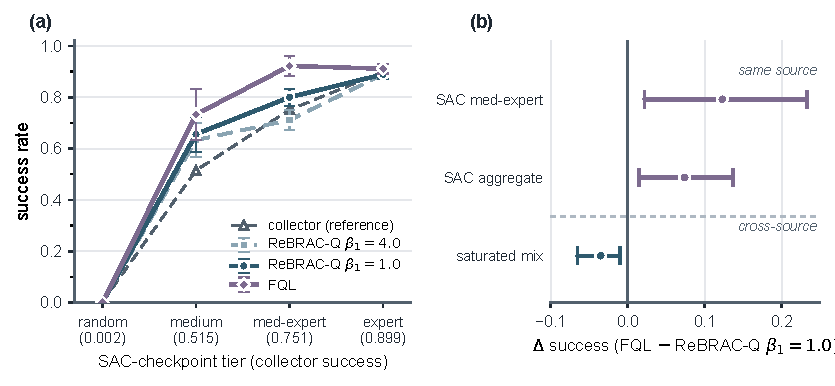
\includegraphics[width=138mm]{figures/fig_ch5_algo_interaction.pdf}
    \caption{算法与数据质量的交互（本章算法比较的核心图）。(a) SAC 检查点四档质量阶梯（横轴括号内为采集器自身成功率）上三个固定配置的终检成功率（三种子均值，误差棒为跨种子标准差；灰色虚线及其三角标记为采集器参考水平）：FQL 恰在非饱和的中段质量区间拉开优势（中等偏专家档 $0.922$ 对 $0.800$），随机档三者皆零、专家档三者同收敛于采集器水平附近。(b) FQL 与 ReBRAC-Q $\beta_1{=}1.0$ 之差及其 $95\%$ 配对自助置信区间：同源的 SAC 中等偏专家档（$+0.123$）与三档聚合（$+0.074$）严格为正，跨源补充的饱和混合单元（$-0.035$）严格为负——方向随数据质量区间翻转，且两侧区间均不含零。虚线分隔的跨源一侧使用不同的数据集与评估协议，仅支撑方向读数，两侧幅度不可直接比较。}
    \label{fig:ch5_algo_interaction}
\end{figure}

跨源数据同时改写了族内判定的强度，也复核了它的机制成分。“$\beta_1=1.0$ 双轴不低于 FQL”由此被界定为饱和高质量区间内的性质而非普适排序——在 SAC 中等偏专家档上 FQL 显著更优。ReBRAC-Q 内部“$\beta_1=1.0$ 不低于 $4.0$”的弱占优则在两族数据的非饱和单元上一致重现（中等偏专家档 $+0.089$，$[+0.011,\,+0.178]$；含噪单模态单元 $+0.235$），饱和单元无检验力但亦无反例（$-0.000$，$[-0.020,\,+0.025]$）——锚定强度机制随数据源保持，改变的只是两算法的相对位置。

\subsection{对中心命题的含义与结论边界}\label{subsec:ch5_algo_implications}

两族证据合起来指向同一个决定因素：离线算法的相对表现不由策略先验的表达力单独决定，而由模仿目标的质量与数据条件的适配决定。数据质量处于尚未逼近上限的中段区间时，流匹配去噪的参照动作滤除了原始动作中不值得模仿的成分，同源对照中 FQL 占优；数据质量高、性能逼近数据上限时，原始动作本身就是好目标，恰当加权的直接模仿与之至少相当，在全场走廊参照一族还沿噪声轴的最坏情形更稳。这兑现中心命题的两个侧面——正向轴的第二途径“使模仿目标与数据质量相适配”在此获得其判别性证据；反向轴的第三项“更具表达力的策略先验”以“不普遍有效”的精确形式成立：生成式先验确有其效，但仅在数据质量落于其去噪能力有事可做的区间内，而算法与数据条件交互的统一收束连同行为约束强度的跨线解释一并留待本章末节。

适用范围沿工况轴有一处明确边界。把噪声轴对照移到临界工况横流基准的探测，在预登记的可学性门控一步即触底：干净示范的采集器自身成功率由亚临界的 $0.985$ 降至 $0.719$，含噪一侧由亚临界的 $0.632$ 更降至 $0.098$，而以其干净示范训练的 ReBRAC-Q $\beta_1=1.0$ 终检仅 $0.14$、越界主导（$78/100$），训练曲线在同等预算下仍于约 $0.09$ 缓升——采集器与离线策略之间约 $58$ 个百分点的塌落，与 \S\ref{sec:ch5_boundary} 在同一临界工况下刻画的单点观测策略侧上限相互印证：两处证据所用的行为约束配置、示范数据与评估集彼此独立，却触及同一边界。算法比较在该工况下未定义，这一边界不削弱本节全部主工况结论。

本节的种子规模须与结论一同引用。全场走廊参照一族每单元两随机种子（干净基准的 FQL 侧四种子）、SAC 一族每档三种子，均低于主线的五种子；支撑机制的两个大效应在此规模下即显著，全部无差异判定只会随种子增加而收紧，翻转的两个方向各有严格不含零的置信区间，但每个效应量的点估计都应按其种子规模解读。承载章级结论的也不是任何单点幅度，而是交互的方向结构本身：算法排序依数据条件而异，其决定因素是模仿目标质量与数据质量的匹配。

\subsection{实施细节与可复现性}\label{subsec:ch5_algo_impl}

数据条件矩阵的四个单元均以表~\ref{tab:ch5_datasets} 中全场走廊参照的亚临界到达导向集为基准，每单元一千回合、$s_0$ 传感、$k=4$ 历史堆叠（观测 $48$ 维），随转移记录特权观测及其后继（\S\ref{subsec:ch5_impl}）：含噪单模态单元在采集时对基准行为策略的动作注入 $\sigma=0.5$ 的高斯噪声（截断 $\pm0.5$）；干净多模态单元由全场走廊参照与目标直指参照各五百回合合成；小噪多模态单元在同一混合构造上注入 $\sigma=0.1$。SAC 检查点四档取自同一条在线训练轨迹（亚临界横流穿越、$s_0$ 传感、$k=4$、到达导向奖励、总预算一百万环境步）的四个阶段检查点（约 $2.5$、$42.5$、$57.5$ 与 $60$ 万环境步），各采集一千回合（采集时保留检查点策略的随机动作采样，而非确定性均值动作），逐档转移规模分别约 $18.0$、$25.1$、$17.1$ 与 $11.5$ 万条；采集器成功率随质量升高，回合均长呈非单调（$180$、$251$、$171$、$115$ 步）——低档以越界早终、中档以超时拖长、高档以快速达标为主，失败模式随档位漂移，是该阶梯覆盖多种数据条件的直接证据。

两算法的超参数均在全部对照前冻结，矩阵与阶梯内不逐单元调参：ReBRAC-Q 取 $(\beta_1,\beta_2)=(4.0,\,2.0)$（沿主线筛查所锁定），FQL 取流积分步数 $10$、蒸馏权重 $\alpha_{\mathrm{FQL}}=1.0$（其原始实现默认值，冻结前未作扫描，\S\ref{subsec:ch5_algo_rescue} 的扫描正为补此不对称）；\S\ref{subsec:ch5_algo_anchor} 的消融与 \S\ref{subsec:ch5_algo_rescue} 的扫描即以此为基线的单变量改动。网络结构与优化器沿 \S\ref{subsec:ch5_method_impl}；每个运行训练二十万梯度步，直接评估训练终点检查点（与 \S\ref{subsec:ch5_boundary_impl} 同口径，对两算法对称）。终检评估分三种：矩阵、消融与扫描用主工况每种子一百回合主评估集（\S\ref{subsec:ch5_eval}）；SAC 四档联合协议用与主评估集同任务分布、独立采样的三十回合固定评估集；小噪多模态单元的跨源补充与配对复核用一百回合主评估集。种子组：矩阵与消融每单元两随机种子，SAC 阶梯每档三随机种子，跨源配对取两族共同的两个随机种子。

统计口径在 \S\ref{subsec:ch5_eval} 的基础上按本节的小种子规模补充。固定评估集使评估抽样噪声成为共模，种子间离散即纯训练种子方差，两样本 $t$ 检验以种子级成功率为样本（每组两种子、自由度 $2$、临界值 $4.30$）；SAC 阶梯的跨档对照以分层配对自助给出区间——以随机种子为第一层、回合为第二层同时重采样（$10^4$ 次）——既保留以种子为主要推断单位的原则，又利用固定评估集的配对性质；跨数据源对照因两侧种子组不同，以两个共同随机种子的逐回合配对自助（$10^4$ 次）给出区间，仅用于方向判定。矩阵各单元的判读门槛、可学性门控与消融预期均在相应实验执行前登记，正文全部区间为 $95\%$ 百分位置信区间。
